\chapter{Implementación en simulador}
\label{ch:simulation-implementation}

El entorno de simulación que nos ofrece \ac{sumo} nos permite recoger la práctica totalidad de información propuesta en la Tabla~\ref{tbl:main-variables} del capítulo \nameref{ch:methodology} con la excepción del entorno.

El problema es que la representación que nos ofrece \ac{sumo} de éste es un conjunto posiciones y tipologías de elementos, de tal manera que podemos acceder a información rápidamente pero de forma muy limitada. Dicho de otro modo, en un entorno real no podemos saber, por ejemplo, que existe un coche en la posición $(x, y, z)$ de unas determinadas dimensiones\sidenote{
	En realidad sí sería posible conseguir esa información con cierto grado de certeza aplicando técnicas de reconocimiento de patrones a las las nubes de puntos. Dichas técnicas son propensas a errores, más aun con la escasa resolución a largas distancias del \ac{lidar} usado en los experimentos, por lo que no han sido consideradas para este trabajo.
}.

Por lo tanto, la solución por la que se ha optado es por la implementación de un \ac{lidar} en el vehículo simulado de tal manera que ofrece una nube de puntos de las mismas características que las capturadas por el \ac{lidar} físico y situado en la misma posición del vehículo. Este \ac{lidar}, a una tasa de \SI{10}{\hertz}, realizará las siguientes operaciones:

\begin{enumerate}
	\item Captura de posición de todos los semáforos situados a un radio $r$ del centro del \ac{lidar} y transformación de éstos a prisma con base cuadrada sitiada a altura \SI{0}{\meter} y con altura de \SI{3}{\meter}.
	\item Captura de posición de todos los vehículos situados a un radio $r$ del centro del \ac{lidar} y transformación de éstos a prismas con las dimensiones que especifiquen sus propiedades.
	\item Cálculo de la nube de puntos colisionando contra los prismas generados.
\end{enumerate}

En el vehículo se han implantado los modelos longitudinales y de cambio de carril\index{lane-change} dentro de un conductor virtual tanto para el sujeto global como para cada uno de los sujetos del experimento y se ha realizado un recorridos de características similares al recorrido del que se obtuvieron los datos del conjunto de test (ver Figura~\ref{fig:sumo-route}).

\begin{marginfigure}
	\centering
	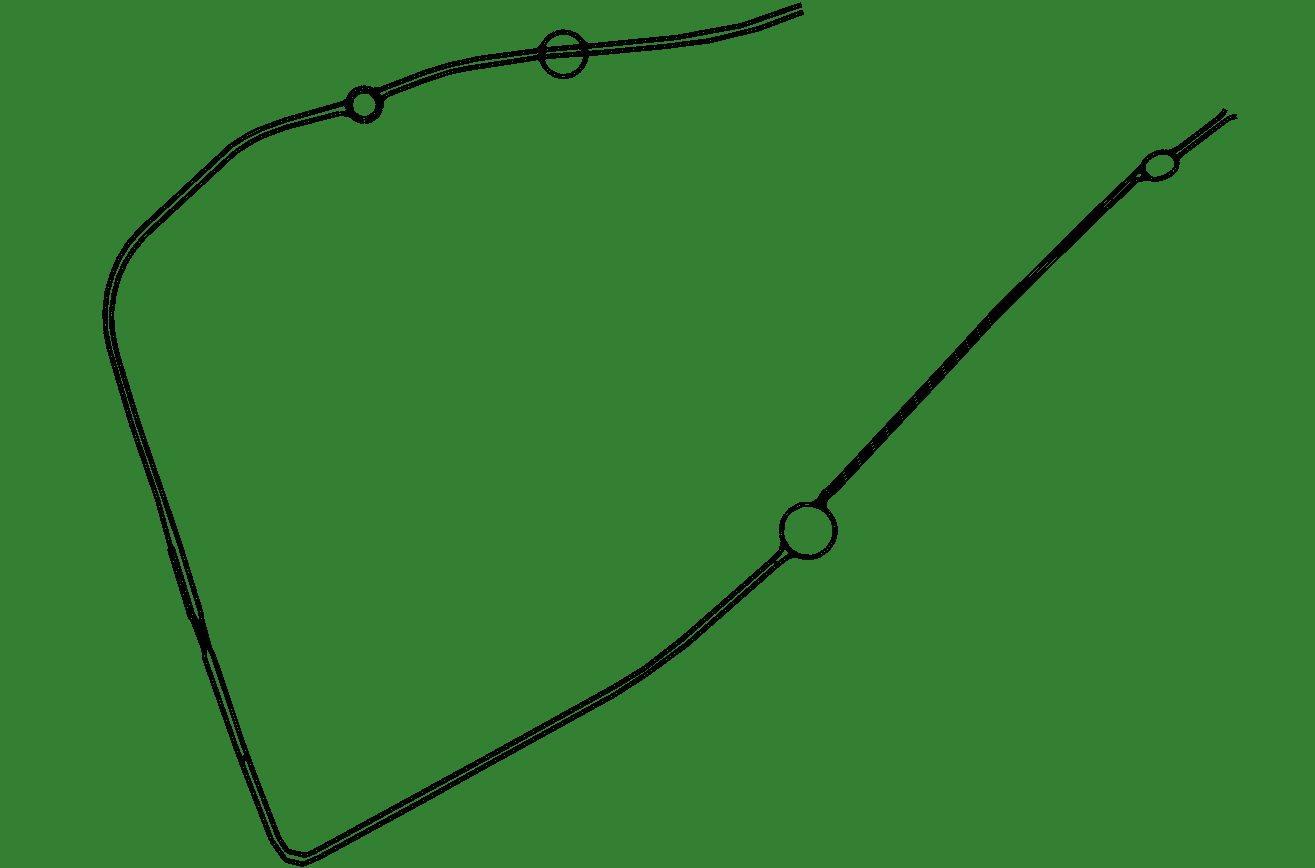
\includegraphics[width=\textwidth]{sumo-route}
	\caption[Circuito de prueba en el entorno virtual]{Circuito generado para recoger los datos de los vehículos circulando con los modelos longitudinal y de cambio de carril implantados.}
	\label{fig:sumo-route}
\end{marginfigure}

La forma por la que se comprobará si los comportamientos son similares es la propuesta en \cite{DiazAlvarez2014} para el comportamiento longitudinal. En la Tabla~\ref{tbl:global-comparison-indicators} se resumen estos valores para el modelo de conducción global y los conductores específicos. La leyenda de indicadores es la siguiente:

\begin{itemize}
	\item $V$. Velocidad instantánea del vehículo.
	\item $AP$/$AN$. Aceleración instantánea positiva y negativa del vehículo.
	\item $JIM$. \textit{Jerk}\sidenote{El \textbf{jerk} es la derivada de la aceleración.} positivo con aceleración positiva, el cual se corresponde con la situación en la que el vehículo está iniciando la marcha (\textit{jerk} de inicio de marcha).
	\item $JLC$. \textit{Jerk} positivo con aceleración negativa, caso que se da cuando se está llegando a la velocidad deseada, por lo que aunque la velocidad sigue aumentando, lo hace en una tasa cada vez más decreciente (\textit{jerk} de llegada a crucero).
	\item $JIF$. \textit{Jerk} negativo con aceleración negativa, cuando el conductor inicia una maniobra de reducción de velocidad (\textit{jerk} de inicio de frenada).
	\item $JFF$. \textit{Jerk} positivo con aceleración negativa, que se corresponde con el momento en el que el conductor está terminando una maniobra de frenada o de reducción de velocidad (\textit{jerk} de fin de frenada).
\end{itemize}

\begin{table*}[!b]
	\centering
	\small
	\caption[Indicadores reales frente a indicadores capturados en simulación][-46em]{Resumen de los indicadores provenientes de los datos de los conductores en los recorridos frente a los valores. En el caso del conjunto global, se ha elegido la media (redondeada a entero en el caso de cambio de carril) de los tres sujetos como estimador de los valores que correspondan para un supuesto conductor medio en ese recorrido. Los valores de los cambios de carril son el numero exacto y no el número de frames que transcurren durante los mismos. Los valores de cambio de carril correspondientes a las simulaciones son la media y la varianza de tres ejecuciones sobre el mismo escenario.}
	\label{tbl:global-comparison-indicators}
	\begin{tabular}{cccccccccc}
		\toprule
		&                   & \multicolumn{2}{c}{$S_A$}    & \multicolumn{2}{c}{$S_1$}          & \multicolumn{2}{c}{$S_2$}        & \multicolumn{2}{c}{\textbf{$S_3$}}        \\
		\multicolumn{2}{l}{}                  & $\mu$     & $\sigma$ & $\mu$    & $\sigma$ & $\mu$     & $\sigma$  & $\mu$    & $\sigma$ \\
		\midrule
		\rowcolor{black!20} \cellcolor{white} \multirow{2}{*}{\textbf{$V$}}   & R. & $3.868$  & $3.515$  & $5.823$  & $5.165$  & $4.246$  & $3.583$  & $2.415$  & $1.834$  \\
		& S. & $3.401$  & $3.003$  & $5.816$  & $4.996$  & $4.111$  & $3.515$  & $2.577$  & $2.050$  \\
		\rowcolor{black!20} \cellcolor{white} \multirow{2}{*}{\textbf{$AP$}}  & R. & $0.082$  & $0.201$  & $0.039$  & $0.029$  & $0.086$  & $0.260$  & $0.084$  & $0.040$  \\
		& S. & $0.042$  & $0.019$  & $0.058$  & $0.029$  & $0.039$  & $0.021$  & $0.060$  & $0.035$  \\
		\rowcolor{black!20} \cellcolor{white} \multirow{2}{*}{\textbf{$AN$}}  & R. & $-0.088$ & $0.144$  & $-0.087$ & $0.048$  & $-0.080$ & $0.173$  & $-0.110$ & $0.041$  \\
		& S. & $-0.050$ & $0.034$  & $-0.053$ & $0.043$  & $-0.039$ & $0.024$  & $-0.065$ & $0.038$  \\
		\rowcolor{black!20} \cellcolor{white} \multirow{2}{*}{\textbf{$JIM$}} & R. & $0.019$  & $0.084$  & $0.011$  & $0.011$  & $0.023$  & $0.112$  & $0.015$  & $0.013$  \\
		& S. & $0.007$  & $0.009$  & $0.009$  & $0.020$  & $0.008$  & $0.011$  & $0.007$  & $0.011$  \\
		\rowcolor{black!20} \cellcolor{white} \multirow{2}{*}{\textbf{$JLC$}} & R. & $0.032$  & $0.127$  & $0.019$  & $0.015$  & $0.039$  & $0.157$  & $0.016$  & $0.016$  \\
		& S. & $0.009$  & $0.018$  & $0.012$  & $0.024$  & $0.010$  & $0.019$  & $0.010$  & $0.017$  \\
		\rowcolor{black!20} \cellcolor{white} \multirow{2}{*}{\textbf{$JIF$}} & R. & $-0.023$ & $0.060$  & $-0.022$ & $0.019$  & $-0.026$ & $0.074$  & $-0.016$ & $0.014$  \\
		& S. & $-0.005$ & $0.010$  & $-0.003$ & $0.010$  & $-0.005$ & $0.008$  & $-0.005$ & $0.013$  \\
		\rowcolor{black!20} \cellcolor{white} \multirow{2}{*}{\textbf{$JFF$}} & R. & $-0.035$ & $0.151$  & $-0.021$ & $0.022$  & $-0.045$ & $0.191$  & $-0.018$ & $0.027$  \\
		& S. & $-0.012$ & $0.023$  & $-0.034$ & $0.047$  & $-0.011$ & $0.188$  & $-0.013$ & $0.027$  \\
		\rowcolor{black!20} \cellcolor{white} \multirow{2}{*}{\textbf{$LC$}}  & R. & $6$     & $1.414$ & $7$     &  -      & $4$     &    -    & $7$     & -       \\
		                                                                      & S. & $2$     & $0$     & $2$     & $0$     & $1$     & $0.471$ & $2$     & $0.816$ \\
		\rowcolor{black!20} \cellcolor{white} \multirow{2}{*}{\textbf{$RC$}}  & R. & $3.333$ & $0.942$ & $2$     &  -      & $4$     &    -    & $4$     &    -    \\
		                                                                      & S. & $1.667$ & $1.700$ & $0.667$ & $0.471$ & $2.333$ & $1.886$ & $0.667$ & $0.943$ \\
		\bottomrule
	\end{tabular}
\end{table*}

Por otro lado, para el comportamiento del modelo de cambio de carril\index{lane-change} se usará el número de éstos que se han producido durante el recorrido, ya que podemos considerar las condiciones similares (i.e. flujo de tráfico moderado en ambas direcciones, misma distancia de recorrido y aproximadamente el mismo número de carriles y semáforos durante el recorrido).

La Tabla~\ref{tbl:global-comparison-indicators} ofrece mucha información, por lo que la comentaremos por partes.

\section{Comportamiento en el modelo longitudinal}

Hemos decidido mostrar los datos de aceleración y \textit{jerk} en el formato de la Figura~\ref{fig:lc-global-comparison-indicators}. Para cada uno de los indicadores se muestran las marcas de cada sujeto de estudio. Cada sujeto tiene una marca diferente asignada para poder ver la diferencia entre ambas.

En el caso de las medias, todos los valores de los sujetos con sus respectivos modelos están muy próximos entre si salvo, quizá, los valores de la aceleración negativa. Lo mismo ocurre con las desviaciones típicas salvo por dos de ellos, el sujeto $S_2$ y el sujeto genérico $S_A$.

Del sujeto genérico es lógico si contamos con que su modelo fue entrenado con los datos del sujeto $S_2$. Si volvemos atrás, al capítulo \nameref{ch:specific-models}, en la Figura~\ref{fig:lm-subjects-comparison} se puede observar que el perfil de aceleración del sujeto $S_2$ es muy irregular, y por tanto es probable que el modelo falle al generalizar esos casos tan específicos.

Del resto de sujetos, sin embargo, no se encuentran demasiadas discrepancias, sino que se mantienen en un nivel similar al del resto de variables.

Podemos concluir que los valores entre simulación y realidad son muy similares entre si, y que por tanto que los conductores simulados se pueden considerar similares a los reales en este comportamiento en concreto.

\begin{figure}[t]
	\centering
	\subfloat[Medias]{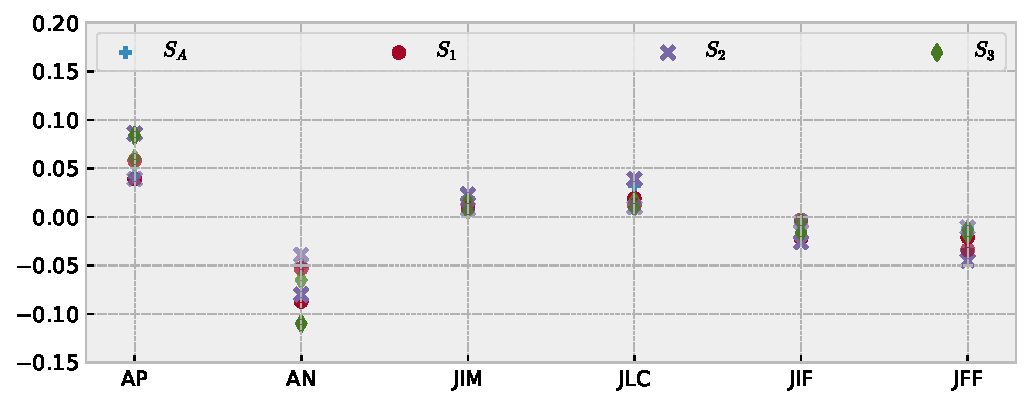
\includegraphics[width=\textwidth]{lc-global-comparison-indicators-means}}\qquad
	\subfloat[Desviaciones típicas]{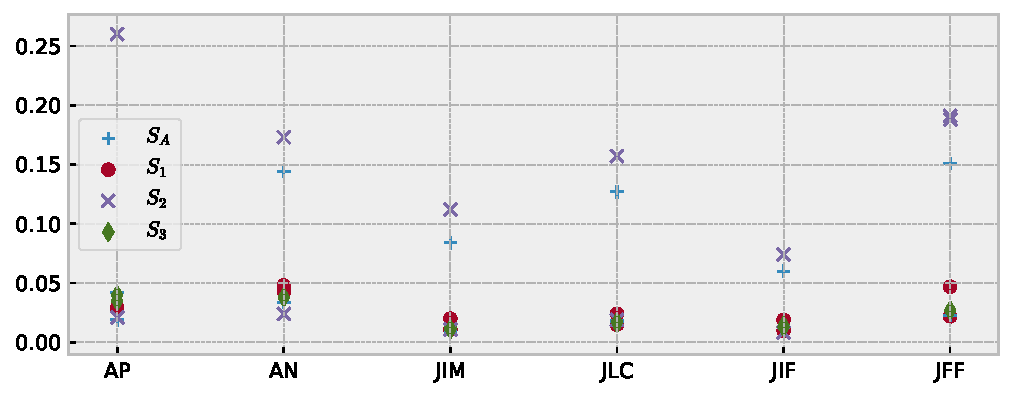
\includegraphics[width=\textwidth]{lc-global-comparison-indicators-stds}}\qquad
	\caption[Medias y desviaciones típicas de los indicadores del modelo longitudinal]{Media y desviación típica de cada uno de los indicadores planteados para el modelo longitudinal. Arriba, las medias y abajo las desviaciones típicas.}
	\label{fig:lc-global-comparison-indicators}
\end{figure}

\section{Comportamiento en el modelo de cambio de carril\index{lane-change}}

En el caso del modelo de cambios de carril, se pueden ver indicios de que el número de cambios de carril en la realidad se mantienen en el mismo rango aproximado que el número de cambios de carril de los modelos estimados, tanto para el general como para los específicos.

Otro detalle es que el número de cambios de carril es menor siempre en el modelo estimado. La razón creo que puede deberse a la baja proporción de cambios de carril respecto a los ejemplos donde éste no existe. Este hecho es muy patente en el caso de los cambios de carril a derecha (fila $RC$ de los indicadores de al tabla~\ref{tbl:global-comparison-indicators}).